\documentclass[hyperref, a4paper]{article}

\usepackage{geometry}
\usepackage{titling}
\usepackage{titlesec}
% No longer needed, since we will use enumitem package
% \usepackage{paralist}
\usepackage{enumitem}
\usepackage{footnote}
\usepackage{enumerate}
\usepackage{amsmath, amssymb, amsthm}
\usepackage{mathtools}
\usepackage{bbm}
\usepackage{cite}
\usepackage{graphicx}
\usepackage{subfigure}
\usepackage{physics}
\usepackage{tensor}
\usepackage{siunitx}
\usepackage[version=4]{mhchem}
\usepackage{tikz}
\usepackage{xcolor}
\usepackage{listings}
\usepackage{autobreak}
\usepackage[ruled, vlined, linesnumbered]{algorithm2e}
\usepackage{nameref,zref-xr}
\zxrsetup{toltxlabel}
\zexternaldocument*[hw2-]{../2/2}[2.pdf]
\usepackage[colorlinks,unicode]{hyperref} % , linkcolor=black, anchorcolor=black, citecolor=black, urlcolor=black, filecolor=black
\usepackage[most]{tcolorbox}
\usepackage{prettyref}

% Page style
\geometry{left=3.18cm,right=3.18cm,top=2.54cm,bottom=2.54cm}
\titlespacing{\paragraph}{0pt}{1pt}{10pt}[20pt]
\setlength{\droptitle}{-5em}
\preauthor{\vspace{-10pt}\begin{center}}
\postauthor{\par\end{center}}

% More compact lists 
\setlist[itemize]{
    itemindent=17pt, 
    leftmargin=1pt,
    listparindent=\parindent,
    parsep=0pt,
}

% Math operators
\DeclareMathOperator{\timeorder}{\mathcal{T}}
\DeclareMathOperator{\diag}{diag}
\DeclareMathOperator{\legpoly}{P}
\DeclareMathOperator{\primevalue}{P}
\DeclareMathOperator{\sgn}{sgn}
\newcommand*{\ii}{\mathrm{i}}
\newcommand*{\ee}{\mathrm{e}}
\newcommand*{\const}{\mathrm{const}}
\newcommand*{\suchthat}{\quad \text{s.t.} \quad}
\newcommand*{\argmin}{\arg\min}
\newcommand*{\argmax}{\arg\max}
\newcommand*{\normalorder}[1]{: #1 :}
\newcommand*{\pair}[1]{\langle #1 \rangle}
\newcommand*{\fd}[1]{\mathcal{D} #1}
\DeclareMathOperator{\bigO}{\mathcal{O}}

% TikZ setting
\usetikzlibrary{arrows,shapes,positioning}
\usetikzlibrary{arrows.meta}
\usetikzlibrary{decorations.markings}
\tikzstyle arrowstyle=[scale=1]
\tikzstyle directed=[postaction={decorate,decoration={markings,
    mark=at position .5 with {\arrow[arrowstyle]{stealth}}}}]
\tikzstyle ray=[directed, thick]
\tikzstyle dot=[anchor=base,fill,circle,inner sep=1pt]

% Algorithm setting
% Julia-style code
\SetKwIF{If}{ElseIf}{Else}{if}{}{elseif}{else}{end}
\SetKwFor{For}{for}{}{end}
\SetKwFor{While}{while}{}{end}
\SetKwProg{Function}{function}{}{end}
\SetArgSty{textnormal}

\newcommand*{\concept}[1]{{\textbf{#1}}}

% Embedded codes
\lstset{basicstyle=\ttfamily,
  showstringspaces=false,
  commentstyle=\color{gray},
  keywordstyle=\color{blue}
}

% Reference formatting
\newrefformat{fig}{Figure~\ref{#1}}

% Color boxes
\tcbuselibrary{skins, breakable, theorems}
\newtcbtheorem[number within=section]{warning}{Warning}%
  {colback=orange!5,colframe=orange!65,fonttitle=\bfseries, breakable}{warn}
\newtcbtheorem[number within=section]{note}{Note}%
  {colback=green!5,colframe=green!65,fonttitle=\bfseries, breakable}{note}
\newtcbtheorem[number within=section]{info}{Info}%
  {colback=blue!5,colframe=blue!65,fonttitle=\bfseries, breakable}{info}

\newenvironment{shelldisplay}{\begin{lstlisting}}{\end{lstlisting}}

\title{Solid State Physics Homework 1}
\author{Jinyuan Wu}

\begin{document}

\maketitle

\paragraph{Problem 1} Consider a 3D Bravais lattice (no basis). One can take all the lattice points and view them as being contained as parallel planes which are called ``lattice planes''. Of course, there are many ways of choosing lattice planes.
(a) If the spacing between lattice planes is $d$ and the volume of the primitive unit cell of the lattice is $V$, show that the areal density of lattice points on a lattice plane is $d / V$.
(b) What set of lattice planes has the highest areal density of lattice points for a BCC lattice? Describe the planes using their (Miller) indices.

\paragraph{Solution} 
\begin{itemize}
\item[(a)] Consider \prettyref{fig:volume-between}. Suppose there are $N$ points in an area $A$
on a certain lattice plane.
The volume between $A$ and its counterpart on an adjacent lattice plane is 
\[
    V_{\text{total}} = A d
\]
Now since there are $N$ points in $A$,
there are $N$ primitive unit cells between $A$ and its counterpart, so 
\[
    V_{\text{total}} = N V.
\]
Thus 
\begin{equation}
    NV = Ad, \quad \text{areal density} \coloneqq \frac{N}{A} = \frac{d}{V}.
\end{equation}
\item[(b)] To maximize the areal density of lattice points is to maximize $d$,
and to maximize $d$ is to pick a lattice plane that is orthogonal to one of the primitive lattice vectors.
By try and error it can be seen that $\{101\}$ is the group of lattice planes we want:
here $d=\sqrt{2}/2$, larger than any other lattice planes.
\end{itemize}

\begin{figure}
    \centering
    

\begin{tikzpicture}[x=0.75pt,y=0.75pt,yscale=-1,xscale=1]
%uncomment if require: \path (0,300); %set diagram left start at 0, and has height of 300

%Straight Lines [id:da40509447135468535] 
\draw [color={rgb, 255:red, 155; green, 155; blue, 155 }  ,draw opacity=1 ] [dash pattern={on 4.5pt off 4.5pt}]  (86,144.04) -- (102,92.04) ;
%Straight Lines [id:da5046748334738116] 
\draw [color={rgb, 255:red, 155; green, 155; blue, 155 }  ,draw opacity=1 ] [dash pattern={on 4.5pt off 4.5pt}]  (73,160) -- (89,108) ;
%Straight Lines [id:da9240421413092696] 
\draw [color={rgb, 255:red, 155; green, 155; blue, 155 }  ,draw opacity=1 ] [dash pattern={on 4.5pt off 4.5pt}]  (63,144.04) -- (79,92.04) ;
%Straight Lines [id:da4809710792018871] 
\draw [color={rgb, 255:red, 155; green, 155; blue, 155 }  ,draw opacity=1 ] [dash pattern={on 4.5pt off 4.5pt}]  (50,160) -- (66,108) ;
%Shape: Parallelogram [id:dp06799371355315431] 
\draw   (98.7,66.04) -- (175,66.04) -- (142.3,108) -- (66,108) -- cycle ;
%Shape: Parallelogram [id:dp7388899093821453] 
\draw   (82.7,118.04) -- (159,118.04) -- (126.3,160) -- (50,160) -- cycle ;
%Straight Lines [id:da8660880194969045] 
\draw    (50,160) -- (73,160) ;
\draw [shift={(73,160)}, rotate = 0] [color={rgb, 255:red, 0; green, 0; blue, 0 }  ][fill={rgb, 255:red, 0; green, 0; blue, 0 }  ][line width=0.75]      (0, 0) circle [x radius= 3.35, y radius= 3.35]   ;
\draw [shift={(50,160)}, rotate = 0] [color={rgb, 255:red, 0; green, 0; blue, 0 }  ][fill={rgb, 255:red, 0; green, 0; blue, 0 }  ][line width=0.75]      (0, 0) circle [x radius= 3.35, y radius= 3.35]   ;
%Straight Lines [id:da5161526563659284] 
\draw    (73,160) -- (96,160) ;
\draw [shift={(96,160)}, rotate = 0] [color={rgb, 255:red, 0; green, 0; blue, 0 }  ][fill={rgb, 255:red, 0; green, 0; blue, 0 }  ][line width=0.75]      (0, 0) circle [x radius= 3.35, y radius= 3.35]   ;
\draw [shift={(73,160)}, rotate = 0] [color={rgb, 255:red, 0; green, 0; blue, 0 }  ][fill={rgb, 255:red, 0; green, 0; blue, 0 }  ][line width=0.75]      (0, 0) circle [x radius= 3.35, y radius= 3.35]   ;
%Straight Lines [id:da39386897512422125] 
\draw    (50,160) -- (63,144.04) ;
\draw [shift={(63,144.04)}, rotate = 309.17] [color={rgb, 255:red, 0; green, 0; blue, 0 }  ][fill={rgb, 255:red, 0; green, 0; blue, 0 }  ][line width=0.75]      (0, 0) circle [x radius= 3.35, y radius= 3.35]   ;
\draw [shift={(50,160)}, rotate = 309.17] [color={rgb, 255:red, 0; green, 0; blue, 0 }  ][fill={rgb, 255:red, 0; green, 0; blue, 0 }  ][line width=0.75]      (0, 0) circle [x radius= 3.35, y radius= 3.35]   ;
%Straight Lines [id:da7187681043638781] 
\draw    (73,160) -- (86,144.04) ;
\draw [shift={(86,144.04)}, rotate = 309.17] [color={rgb, 255:red, 0; green, 0; blue, 0 }  ][fill={rgb, 255:red, 0; green, 0; blue, 0 }  ][line width=0.75]      (0, 0) circle [x radius= 3.35, y radius= 3.35]   ;
\draw [shift={(73,160)}, rotate = 309.17] [color={rgb, 255:red, 0; green, 0; blue, 0 }  ][fill={rgb, 255:red, 0; green, 0; blue, 0 }  ][line width=0.75]      (0, 0) circle [x radius= 3.35, y radius= 3.35]   ;
%Straight Lines [id:da0904767212465516] 
\draw [color={rgb, 255:red, 155; green, 155; blue, 155 }  ,draw opacity=1 ]   (152,118.04) -- (208,118.04) ;
%Straight Lines [id:da8112713117460995] 
\draw [color={rgb, 255:red, 155; green, 155; blue, 155 }  ,draw opacity=1 ]   (175,66.04) -- (208,66.04) ;
%Straight Lines [id:da8711718170026372] 
\draw [color={rgb, 255:red, 155; green, 155; blue, 155 }  ,draw opacity=1 ] [dash pattern={on 4.5pt off 4.5pt}]  (190,68.04) -- (190,116.04) ;
\draw [shift={(190,118.04)}, rotate = 270] [fill={rgb, 255:red, 155; green, 155; blue, 155 }  ,fill opacity=1 ][line width=0.08]  [draw opacity=0] (12,-3) -- (0,0) -- (12,3) -- cycle    ;
\draw [shift={(190,66.04)}, rotate = 90] [fill={rgb, 255:red, 155; green, 155; blue, 155 }  ,fill opacity=1 ][line width=0.08]  [draw opacity=0] (12,-3) -- (0,0) -- (12,3) -- cycle    ;
%Straight Lines [id:da737172554421827] 
\draw    (63,144.04) -- (86,144.04) ;
\draw [shift={(86,144.04)}, rotate = 0] [color={rgb, 255:red, 0; green, 0; blue, 0 }  ][fill={rgb, 255:red, 0; green, 0; blue, 0 }  ][line width=0.75]      (0, 0) circle [x radius= 3.35, y radius= 3.35]   ;
\draw [shift={(63,144.04)}, rotate = 0] [color={rgb, 255:red, 0; green, 0; blue, 0 }  ][fill={rgb, 255:red, 0; green, 0; blue, 0 }  ][line width=0.75]      (0, 0) circle [x radius= 3.35, y radius= 3.35]   ;
%Straight Lines [id:da9264832738509183] 
\draw    (66,108) -- (89,108) ;
\draw [shift={(89,108)}, rotate = 0] [color={rgb, 255:red, 0; green, 0; blue, 0 }  ][fill={rgb, 255:red, 0; green, 0; blue, 0 }  ][line width=0.75]      (0, 0) circle [x radius= 3.35, y radius= 3.35]   ;
\draw [shift={(66,108)}, rotate = 0] [color={rgb, 255:red, 0; green, 0; blue, 0 }  ][fill={rgb, 255:red, 0; green, 0; blue, 0 }  ][line width=0.75]      (0, 0) circle [x radius= 3.35, y radius= 3.35]   ;
%Straight Lines [id:da5329200824589426] 
\draw    (89,108) -- (112,108) ;
\draw [shift={(112,108)}, rotate = 0] [color={rgb, 255:red, 0; green, 0; blue, 0 }  ][fill={rgb, 255:red, 0; green, 0; blue, 0 }  ][line width=0.75]      (0, 0) circle [x radius= 3.35, y radius= 3.35]   ;
\draw [shift={(89,108)}, rotate = 0] [color={rgb, 255:red, 0; green, 0; blue, 0 }  ][fill={rgb, 255:red, 0; green, 0; blue, 0 }  ][line width=0.75]      (0, 0) circle [x radius= 3.35, y radius= 3.35]   ;
%Straight Lines [id:da2773689191142634] 
\draw    (66,108) -- (79,92.04) ;
\draw [shift={(79,92.04)}, rotate = 309.17] [color={rgb, 255:red, 0; green, 0; blue, 0 }  ][fill={rgb, 255:red, 0; green, 0; blue, 0 }  ][line width=0.75]      (0, 0) circle [x radius= 3.35, y radius= 3.35]   ;
\draw [shift={(66,108)}, rotate = 309.17] [color={rgb, 255:red, 0; green, 0; blue, 0 }  ][fill={rgb, 255:red, 0; green, 0; blue, 0 }  ][line width=0.75]      (0, 0) circle [x radius= 3.35, y radius= 3.35]   ;
%Straight Lines [id:da10009334559985272] 
\draw    (89,108) -- (102,92.04) ;
\draw [shift={(102,92.04)}, rotate = 309.17] [color={rgb, 255:red, 0; green, 0; blue, 0 }  ][fill={rgb, 255:red, 0; green, 0; blue, 0 }  ][line width=0.75]      (0, 0) circle [x radius= 3.35, y radius= 3.35]   ;
\draw [shift={(89,108)}, rotate = 309.17] [color={rgb, 255:red, 0; green, 0; blue, 0 }  ][fill={rgb, 255:red, 0; green, 0; blue, 0 }  ][line width=0.75]      (0, 0) circle [x radius= 3.35, y radius= 3.35]   ;
%Straight Lines [id:da20112614980324728] 
\draw    (79,92.04) -- (102,92.04) ;
\draw [shift={(102,92.04)}, rotate = 0] [color={rgb, 255:red, 0; green, 0; blue, 0 }  ][fill={rgb, 255:red, 0; green, 0; blue, 0 }  ][line width=0.75]      (0, 0) circle [x radius= 3.35, y radius= 3.35]   ;
\draw [shift={(79,92.04)}, rotate = 0] [color={rgb, 255:red, 0; green, 0; blue, 0 }  ][fill={rgb, 255:red, 0; green, 0; blue, 0 }  ][line width=0.75]      (0, 0) circle [x radius= 3.35, y radius= 3.35]   ;

% Text Node
\draw (192,92.04) node [anchor=west] [inner sep=0.75pt]    {$d$};
% Text Node
\draw (114,75.4) node [anchor=north west][inner sep=0.75pt]    {$A$};
% Text Node
\draw (43,115.4) node [anchor=north west][inner sep=0.75pt]    {$V$};
% Text Node
\draw (51,172) node [anchor=north west][inner sep=0.75pt]   [align=left] {$\displaystyle N$ points};


\end{tikzpicture}

    \caption{The volume between two areas on adjacent lattice planes}
    \label{fig:volume-between}
\end{figure}

\paragraph{Problem 2} Problem 1 of Chapter 4 of A\&M. Assume the side of the cubes are one unit long.
In each of the following cases indicate whether the structure is a Bravais lattice. If it is, give three primitive vectors; if it is not, describe it as a Bravais lattice with as small as possible a basis.
(a) Base-centered cubic (simple cubic with additional points in the centers of the horizontal faces of the cubic cell).
(b) Side-centered cubic (simple cubic with additional points in the centers of the vertical faces of the cubic cell).
(c) Edge-centered cubic (simple cubic with additional points at the midpoints of the lines joining nearest neighbors).

\paragraph{Solution} 
Below I use the side length of the so-called cubes as the length unit.
\begin{itemize}
\item[(a)] Based-centered cubic is a Bravais lattice but the name is not on the list of 14. 
It is not really cubic, 
because it doesn't have the rotational symmetry around the $x$ and $y$ axes.
It's actually a simple tetragonal lattice with $a= 1 / \sqrt{2}, c = 1$, and
the primitive vectors are 
\begin{equation}
    \vb*{a}_1 = (1/2, -1/2, 0), \quad \vb*{a}_2 = (1/2, 1/2, 0), \quad \vb*{a}_3 = (0, 0, 1).
    \label{eq:based-centered-cubic-vector}
\end{equation}
\item[(b)] Similar to the first case, 
side-centered cubic is also a Bravais lattice but not cubic,
because it also doesn't have the rotational symmetry around the $x$ and $y$ axes
and therefore is not really ``cubic''.
It's actually a body-centered tetragonal lattice with $a= 1 / \sqrt{2}, c = 1$.
The primitive vectors are the same with \eqref{eq:based-centered-cubic-vector}.
\item[(c)] The edge-centered cubic lattice has the symmetry of a cube and therefore has to be a cubic lattice.
By counting the number of lattice points, 
we find \prettyref{fig:unit-cell-edge-centered} shows one unit cell.
No translation symmetry is able to turn one of the points into another,
so the unit cell is actually a primitive one.
Thus the edge-centered cubic lattice is actually a simple cubic lattice: 
in each primitive unit cell,
there are four points.
So the edge-centered cubic lattice is not a Bravais lattice.
It's the simple cubic lattice plus the basis shown as black (or red, or blue) in 
\prettyref{fig:unit-cell-edge-centered}.
\end{itemize}

\begin{figure}
    \centering
    


\begin{tikzpicture}[x=0.75pt,y=0.75pt,yscale=-1,xscale=1]
%uncomment if require: \path (0,300); %set diagram left start at 0, and has height of 300

%Shape: Cube [id:dp27906377889622136] 
\draw   (100,124.66) -- (129.29,95.38) -- (198,95.38) -- (198,163.71) -- (168.71,193) -- (100,193) -- cycle ; \draw   (198,95.38) -- (168.71,124.66) -- (100,124.66) ; \draw   (168.71,124.66) -- (168.71,193) ;
%Straight Lines [id:da8949678203128855] 
\draw    (198,95.38) -- (198,163.71) ;
%Straight Lines [id:da49535075513935123] 
\draw  [dash pattern={on 4.5pt off 4.5pt}]  (129.29,95.38) -- (129.29,163.71) ;
%Straight Lines [id:da9925075456381425] 
\draw  [dash pattern={on 4.5pt off 4.5pt}]  (198,163.71) -- (129.29,163.71) ;
%Straight Lines [id:da4763063388834874] 
\draw  [dash pattern={on 4.5pt off 4.5pt}]  (100,193) -- (129.29,163.71) ;
%Straight Lines [id:da6235209425906698] 
\draw    (168.71,124.66) ;
\draw [shift={(168.71,124.66)}, rotate = 0] [color={rgb, 255:red, 0; green, 0; blue, 0 }  ][fill={rgb, 255:red, 0; green, 0; blue, 0 }  ][line width=0.75]      (0, 0) circle [x radius= 3.35, y radius= 3.35]   ;
%Straight Lines [id:da6830253639832535] 
\draw    (136,124.66) ;
\draw [shift={(136,124.66)}, rotate = 0] [color={rgb, 255:red, 0; green, 0; blue, 0 }  ][fill={rgb, 255:red, 0; green, 0; blue, 0 }  ][line width=0.75]      (0, 0) circle [x radius= 3.35, y radius= 3.35]   ;
%Straight Lines [id:da3555449792412686] 
\draw    (182.71,110.66) ;
\draw [shift={(182.71,110.66)}, rotate = 0] [color={rgb, 255:red, 0; green, 0; blue, 0 }  ][fill={rgb, 255:red, 0; green, 0; blue, 0 }  ][line width=0.75]      (0, 0) circle [x radius= 3.35, y radius= 3.35]   ;
%Straight Lines [id:da30048729914335426] 
\draw    (168.71,157.66) ;
\draw [shift={(168.71,157.66)}, rotate = 0] [color={rgb, 255:red, 0; green, 0; blue, 0 }  ][fill={rgb, 255:red, 0; green, 0; blue, 0 }  ][line width=0.75]      (0, 0) circle [x radius= 3.35, y radius= 3.35]   ;
%Straight Lines [id:da39538770796014844] 
\draw [color={rgb, 255:red, 208; green, 2; blue, 27 }  ,draw opacity=1 ]   (99.71,124.66) ;
\draw [shift={(99.71,124.66)}, rotate = 0] [color={rgb, 255:red, 208; green, 2; blue, 27 }  ,draw opacity=1 ][fill={rgb, 255:red, 208; green, 2; blue, 27 }  ,fill opacity=1 ][line width=0.75]      (0, 0) circle [x radius= 3.35, y radius= 3.35]   ;
%Straight Lines [id:da5417236582392115] 
\draw [color={rgb, 255:red, 208; green, 2; blue, 27 }  ,draw opacity=1 ]   (67,124.66) ;
\draw [shift={(67,124.66)}, rotate = 0] [color={rgb, 255:red, 208; green, 2; blue, 27 }  ,draw opacity=1 ][fill={rgb, 255:red, 208; green, 2; blue, 27 }  ,fill opacity=1 ][line width=0.75]      (0, 0) circle [x radius= 3.35, y radius= 3.35]   ;
%Straight Lines [id:da7317973769989081] 
\draw [color={rgb, 255:red, 208; green, 2; blue, 27 }  ,draw opacity=1 ]   (113.71,110.66) ;
\draw [shift={(113.71,110.66)}, rotate = 0] [color={rgb, 255:red, 208; green, 2; blue, 27 }  ,draw opacity=1 ][fill={rgb, 255:red, 208; green, 2; blue, 27 }  ,fill opacity=1 ][line width=0.75]      (0, 0) circle [x radius= 3.35, y radius= 3.35]   ;
%Straight Lines [id:da6579080343176826] 
\draw [color={rgb, 255:red, 208; green, 2; blue, 27 }  ,draw opacity=1 ]   (99.71,157.66) ;
\draw [shift={(99.71,157.66)}, rotate = 0] [color={rgb, 255:red, 208; green, 2; blue, 27 }  ,draw opacity=1 ][fill={rgb, 255:red, 208; green, 2; blue, 27 }  ,fill opacity=1 ][line width=0.75]      (0, 0) circle [x radius= 3.35, y radius= 3.35]   ;

%Straight Lines [id:da3609355877334228] 
\draw [color={rgb, 255:red, 74; green, 144; blue, 226 }  ,draw opacity=1 ]   (168.71,192.66) ;
\draw [shift={(168.71,192.66)}, rotate = 0] [color={rgb, 255:red, 74; green, 144; blue, 226 }  ,draw opacity=1 ][fill={rgb, 255:red, 74; green, 144; blue, 226 }  ,fill opacity=1 ][line width=0.75]      (0, 0) circle [x radius= 3.35, y radius= 3.35]   ;
%Straight Lines [id:da7479710636712822] 
\draw [color={rgb, 255:red, 74; green, 144; blue, 226 }  ,draw opacity=1 ]   (136,192.66) ;
\draw [shift={(136,192.66)}, rotate = 0] [color={rgb, 255:red, 74; green, 144; blue, 226 }  ,draw opacity=1 ][fill={rgb, 255:red, 74; green, 144; blue, 226 }  ,fill opacity=1 ][line width=0.75]      (0, 0) circle [x radius= 3.35, y radius= 3.35]   ;
%Straight Lines [id:da2086207673220617] 
\draw [color={rgb, 255:red, 74; green, 144; blue, 226 }  ,draw opacity=1 ]   (182.71,178.66) ;
\draw [shift={(182.71,178.66)}, rotate = 0] [color={rgb, 255:red, 74; green, 144; blue, 226 }  ,draw opacity=1 ][fill={rgb, 255:red, 74; green, 144; blue, 226 }  ,fill opacity=1 ][line width=0.75]      (0, 0) circle [x radius= 3.35, y radius= 3.35]   ;
%Straight Lines [id:da8842065819921627] 
\draw [color={rgb, 255:red, 74; green, 144; blue, 226 }  ,draw opacity=1 ]   (168.71,225.66) ;
\draw [shift={(168.71,225.66)}, rotate = 0] [color={rgb, 255:red, 74; green, 144; blue, 226 }  ,draw opacity=1 ][fill={rgb, 255:red, 74; green, 144; blue, 226 }  ,fill opacity=1 ][line width=0.75]      (0, 0) circle [x radius= 3.35, y radius= 3.35]   ;

%Straight Lines [id:da3182715597136758] 
\draw [color={rgb, 255:red, 80; green, 227; blue, 194 }  ,draw opacity=1 ]   (100.71,192.66) ;
\draw [shift={(100.71,192.66)}, rotate = 0] [color={rgb, 255:red, 80; green, 227; blue, 194 }  ,draw opacity=1 ][fill={rgb, 255:red, 80; green, 227; blue, 194 }  ,fill opacity=1 ][line width=0.75]      (0, 0) circle [x radius= 3.35, y radius= 3.35]   ;
%Straight Lines [id:da09238987837864565] 
\draw [color={rgb, 255:red, 80; green, 227; blue, 194 }  ,draw opacity=1 ]   (68,192.66) ;
\draw [shift={(68,192.66)}, rotate = 0] [color={rgb, 255:red, 80; green, 227; blue, 194 }  ,draw opacity=1 ][fill={rgb, 255:red, 80; green, 227; blue, 194 }  ,fill opacity=1 ][line width=0.75]      (0, 0) circle [x radius= 3.35, y radius= 3.35]   ;
%Straight Lines [id:da024868637558111972] 
\draw [color={rgb, 255:red, 80; green, 227; blue, 194 }  ,draw opacity=1 ]   (114.71,178.66) ;
\draw [shift={(114.71,178.66)}, rotate = 0] [color={rgb, 255:red, 80; green, 227; blue, 194 }  ,draw opacity=1 ][fill={rgb, 255:red, 80; green, 227; blue, 194 }  ,fill opacity=1 ][line width=0.75]      (0, 0) circle [x radius= 3.35, y radius= 3.35]   ;
%Straight Lines [id:da6333331707155729] 
\draw [color={rgb, 255:red, 80; green, 227; blue, 194 }  ,draw opacity=1 ]   (100.71,225.66) ;
\draw [shift={(100.71,225.66)}, rotate = 0] [color={rgb, 255:red, 80; green, 227; blue, 194 }  ,draw opacity=1 ][fill={rgb, 255:red, 80; green, 227; blue, 194 }  ,fill opacity=1 ][line width=0.75]      (0, 0) circle [x radius= 3.35, y radius= 3.35]   ;

%Straight Lines [id:da5979371349789433] 
\draw [color={rgb, 255:red, 208; green, 2; blue, 27 }  ,draw opacity=1 ]   (165.71,102.66) -- (99,102.66) ;
\draw [shift={(97,102.66)}, rotate = 360] [fill={rgb, 255:red, 208; green, 2; blue, 27 }  ,fill opacity=1 ][line width=0.08]  [draw opacity=0] (12,-3) -- (0,0) -- (12,3) -- cycle    ;
%Straight Lines [id:da9138705372611224] 
\draw [color={rgb, 255:red, 80; green, 227; blue, 194 }  ,draw opacity=1 ]   (161.71,119.66) -- (94.42,186.59) ;
\draw [shift={(93,188)}, rotate = 315.16] [fill={rgb, 255:red, 80; green, 227; blue, 194 }  ,fill opacity=1 ][line width=0.08]  [draw opacity=0] (12,-3) -- (0,0) -- (12,3) -- cycle    ;
%Straight Lines [id:da42187668274599144] 
\draw [color={rgb, 255:red, 74; green, 144; blue, 226 }  ,draw opacity=1 ]   (192.71,124.66) -- (192.71,191) ;
\draw [shift={(192.71,193)}, rotate = 270] [fill={rgb, 255:red, 74; green, 144; blue, 226 }  ,fill opacity=1 ][line width=0.08]  [draw opacity=0] (12,-3) -- (0,0) -- (12,3) -- cycle    ;




\end{tikzpicture}

    \caption{One unit cell of a edge centered cubic lattice}
    \label{fig:unit-cell-edge-centered}
\end{figure}

\paragraph{Problem 3} Problem 5(b) of Chapter 4 of A\&M.
Sodium transforms from bcc to hcp at about 23K (the ``martensitic'' transformation). Assuming that the density remains fixed through this transition, find the lattice constant $a$ of the hexagonal phase, given that $a=\SI{4.23}{\angstrom}$ in the cubic phase and that the $c / a$ ratio is indistinguishable from its ideal value.

\paragraph{Solution} In each conventional cell of the bcc lattice, 
there are 2 lattice points, and so is the case for hcp.
The volume of a conventional cell of the bcc lattice is $a^3$.
In the hcp lattice, $c = 2 \sqrt{6} a / 3$,
so the volume is 
\[
    \frac{\sqrt{3}}{2} a^2 \times c = \sqrt{2} a^3.
\]
So to keep the density invariant,
\[
    \sqrt{2} a_\text{hcp}^3 = a_{\text{bcc}}^3,
\]
and 
\begin{equation}
    a_{\text{hcp}} = 2^{-1/6} a_{\text{bcc}} = \SI{3.77}{\angstrom}.
\end{equation}

\paragraph{Problem 4} $\mathrm{SrTiO}_3$ is an important metal oxide in its own right and is also used as a substrate on which other metal oxides, such as high temperature superconductors, are
grown. Its unit cell structure is shown below. Its crystal system is cubic. Assume the sides of the cube are along the $x, y$ and $z$ axes and are of unit length.

\begin{center}
    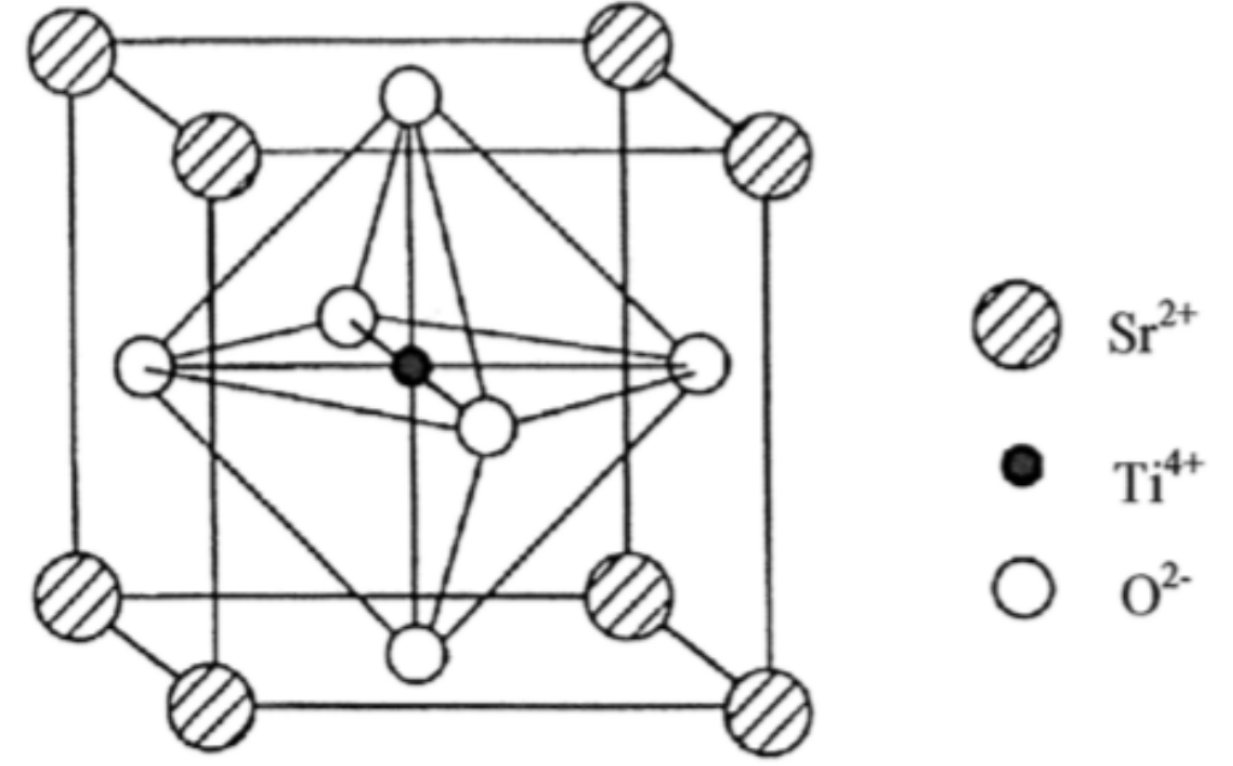
\includegraphics[width=0.5\textwidth]{lattices/SrTiO3.PNG}
\end{center}

\paragraph{Solution} \begin{itemize}
\item[(a)] There is only one Ti atom in the cube given, 
and obviously it's impossible to use a translation symmetry operation 
to turn one atom into another in the cube.
The lattice is a simple cubic lattice,
and the primitive lattice vectors are 
\begin{equation}
    \vb*{a}_1 = (1, 0, 0), \quad \vb*{a}_2 = (0, 1, 0), \quad \vb*{a}_3 = (0, 0, 1).
\end{equation}
\item[(b)] There are five: $1/4 \times 4 = 1$ Sr atom, $1$ Ti atom, and 
$1/2 \times 6 = 3$ O atoms.
The coordinates of the Ti atom are $(1/2, 1/2, 1/2)$.
The coordinates of the Sr atom are $(0, 0, 0)$.
The coordinates of the O atoms are $(1/2, 1/2, 0), (0, 1/2, 1/2), (1/2, 0, 1/2)$.
\item[(c)] The nearest neighbors of a Sr atom are 12 Ti atoms.
The nearest neighbors of a Ti atom are 6 O atoms.
The nearest neighbors of an O atom are 2 Ti atoms.
\end{itemize}

\paragraph{Problem 5} How many $\langle 110 \rangle$ directions are contained in the (111) plane of the BCC structure? List all the specific directions. This problem uses conventional (non-primitive) cubic unit vectors.

\paragraph{Solution} There are 12 $\langle 110 \rangle$ directions:
\[
    [110], [1 \bar{1} 0], [\bar{1} 1 0], [\bar{1} \bar{1} 0], 
    [101], [1 0 \bar{1}], [\bar{1} 0 1], [\bar{1} 0 \bar{1}],
    [011], [0 1 \bar{1}], [0 \bar{1} 1], [0 \bar{1} \bar{1}].
\]
They can be obtained by first applying reflection operations along the $xz$ and $yz$ planes
and then rotating.
Since we are in Cartesian coordinates, 
$(1, 1, 1)$ is just a normal vector of the (111) plane.
By direct calculation of inner product, the following 6 directions are in the (111) plane 
(i.e. orthogonal to its normal vector):
\[
    [1 \bar{1} 0], [\bar{1} 1 0], [1 0 \bar{1}], [\bar{1} 0 1], [0 1 \bar{1}], [0 \bar{1} 1].
\]

\end{document}